\begin{figure}[h!]
    \centering
    \caption{Probability of being a head of household, by income decile}
    \label{fig:ahs_hhead}

    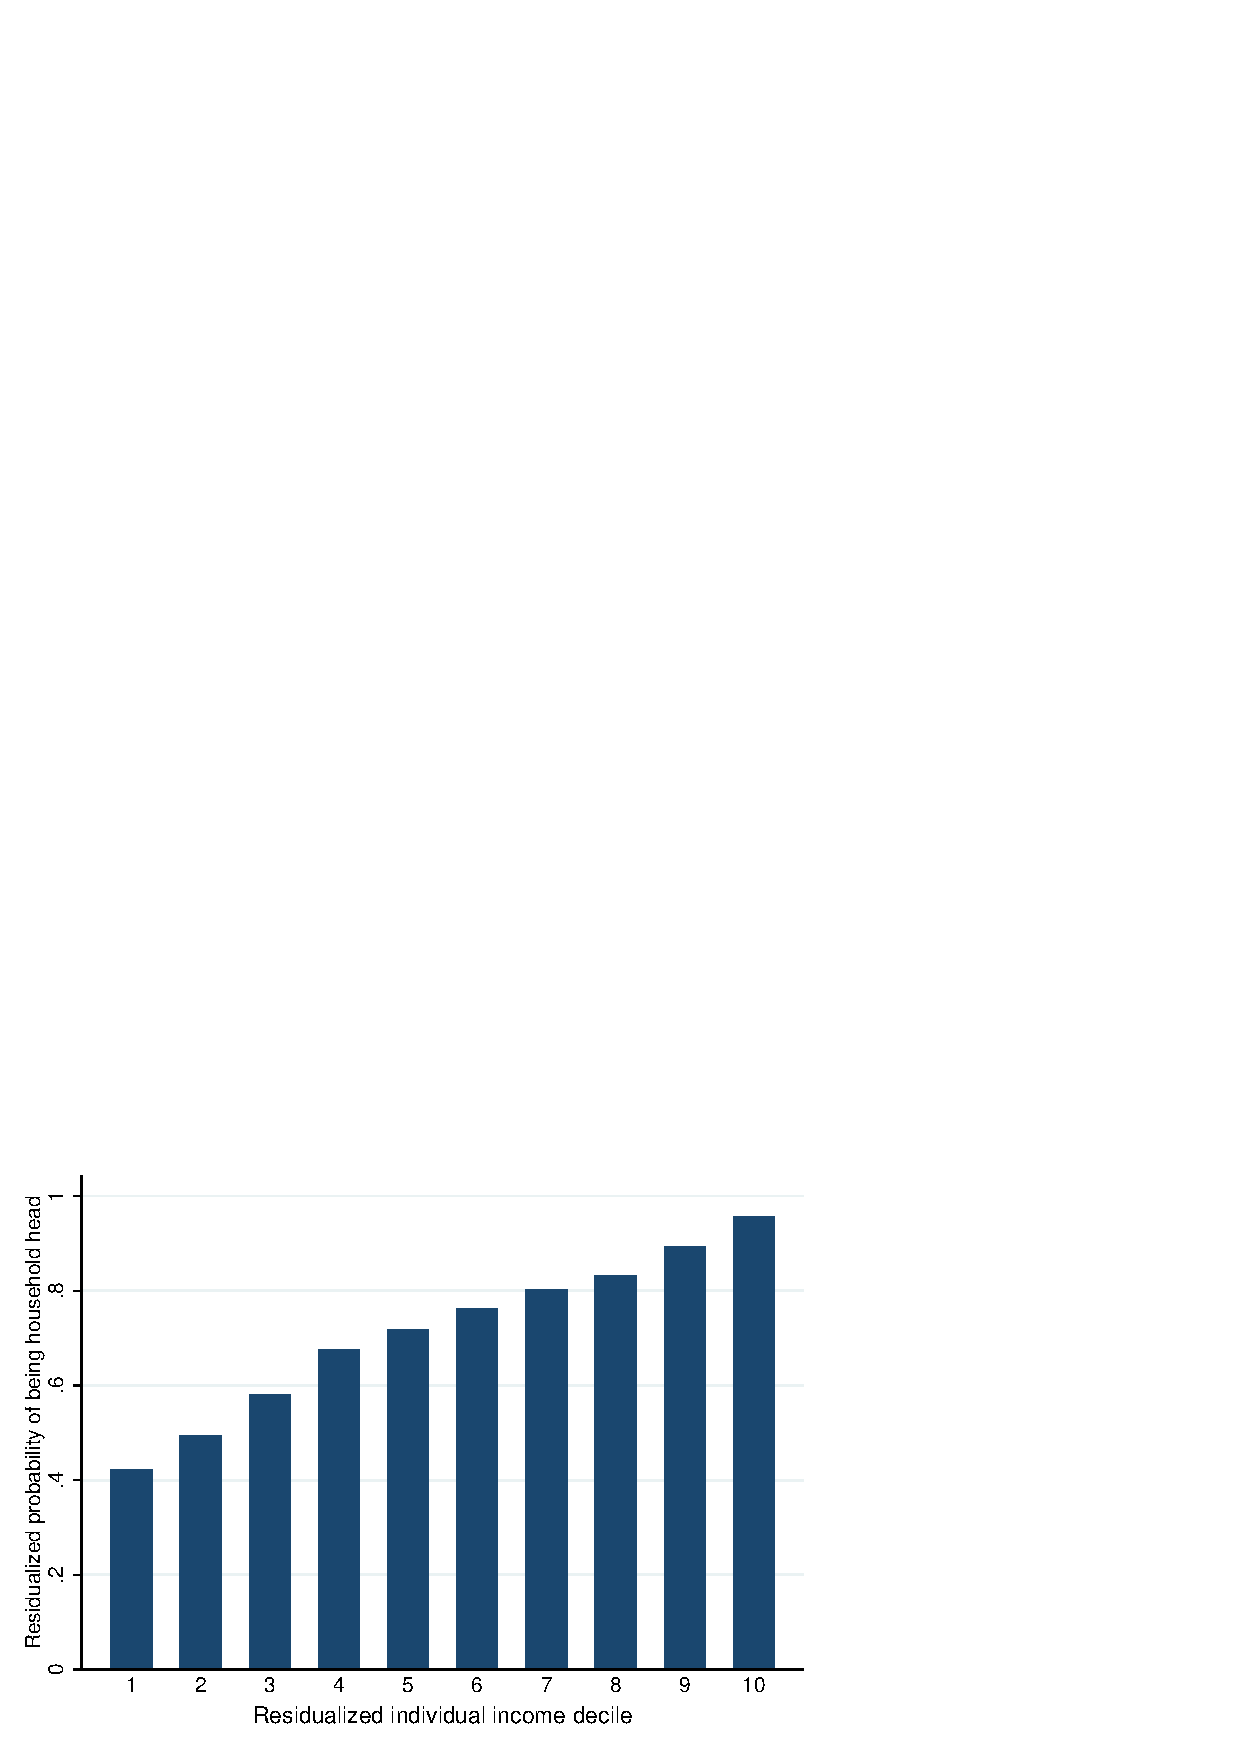
\includegraphics[width = .75\textwidth]{ahs/output/sh_hh_head}
    
    \begin{minipage}{.95\textwidth} \footnotesize
        \vspace{3mm}
        Notes: Data are from the 2011 and 2013 American Housing Surveys.
        The figure shows the probability that an individual is a head of
        household, by individual income decile.
        We construct the figure as follows.
        First, we residualize the variable in the y-axis and individual income 
        by SMSA indicators, the closest analogue of CBSAs available in the data.
        Second, we construct deciles of the residualized individual income 
        variable.
        Finally, we take the average of the residualized y-variable within each 
        decile.
        Individuals that do not work are excluded from the figure.
    \end{minipage}
\end{figure}
